آرزو و بهار در یک بازی مجموع‌صفر شرکت می‌کنند. آرزو از یک دسته کارت که آن‌ها را نمی‌بیند یکی را خارج می‌کند و رنگ آن را می‌بیند ولی به بهار نشان نمی‌دهد. کارت‌ها یا قرمز هستند یا سیاه. هر کدام از این دو نفر در ابتدا یک دلار روی رنگ کارت شرط‌بندی کرده‌اند. پس از آن که آرزو رنگ کارت را دید می‌تواند دو اقدام متفاوت انجام بدهد.
اگر اقدامی که آرزو انجام می‌دهد check باشد، رنگ کارت به بهار نشان داده می‌شود و بازی تمام می‌شود. اگر کارت قرمز باشد، دو دلار به آرزو می‌رسد و در غیر این صورت بهار آن را می‌برد. اگر اقدامی که آرزو انجام می‌دهد raise باشد، یعنی تصمیم گرفته است شرط را دو برابر کند. در این حالت نوبت به تصمیم‌گیری بهار می‌رسد که او هم دو اقدام را در دسترس دارد.
اگر اقدامی که بهار انجام می‌دهد pass باشد یعنی دو برابر شدن جایزه را نپذیرفته است. در این حالت بدون آن که کارت به بهار نشان داده شود بازی به پایان می‌رسد و دو دلار هم مال آرزو می‌شود. اگر اقدامی که بهار انجام می‌دهد meet باشد، یعنی دو برابر شدن جایزه را پذیرفته است. در این حالت رنگ کارت به بهار نشان داده می‌شود و بازی تمام می‌شود. اگر قرمز باشد، چهار دلار به آرزو می‌رسد و در غیر این صورت بهار آن را می‌برد.
فرض کنید احتمال قرمز بودن کارت برابر با
$r$
باشد.
\begin{center}
    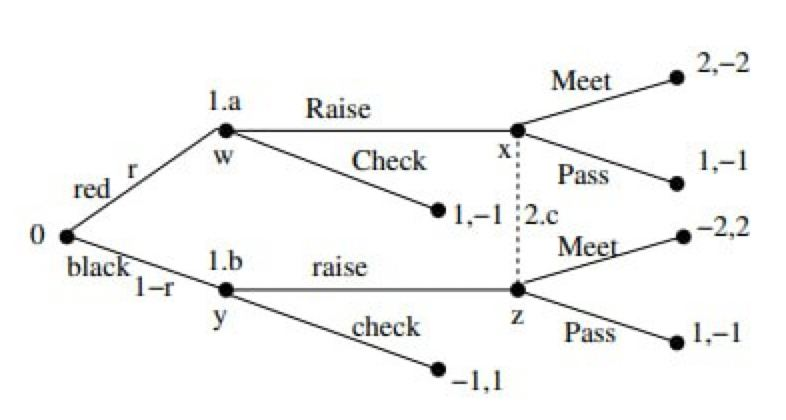
\includegraphics[width=0.6\linewidth]{pics/image5}
\end{center}
\textbf{الف)}
امید ریاضی سود هر نفر را محاسبه کنید.
\vspace{5pt}

\textbf{ب)}
اگر
$r < \frac{3}{4}$
یک تعادل نش ترکیبی بیابید.